\subsection{Conceptos MVC}

El Modelo Vista Controlador (MVC) es un patrón arquitectónico de software que divide una aplicación en tres elementos interconectados, separando la representación interna de la información, como se muestra al usuario y donde se hacen cómputos con esa información respectivamente. \bigskip

Para esta práctica, se ha decidido modificar parcialmente este patrón al implementar la comunicación entre los módulos mediante un sistema de peticiones. Por ende, encontramos 4 módulos en nuestro MVC: Modelo, Vista, Controlador y Hub. Este último se encargará de gestionar toda la comunicación. \bigskip

Esta decisión de modificación del MVC ha sido respaldada por la facilidad que obtenemos de escalar el patrón, permitiendo crear tantos módulos como queramos. Esto permitiría que, si en un futuro se quisiera añadir otro controlador en otro lenguaje de programación o encapsular controladores por funcionalidad, el único cambio a efectuar ocurriría en el hub.\bigskip

% El programa principal ejecutará la librería Mesurament.jar para medir un RATIO. Además, se ejecutará una configuración predeterminada del programa a partir de un documento de texto. Creando las partes del programa como interficies y conectando el patrón mediante punteros.  \bigskip

A continuación se explicarán cada uno de los módulos.

\section{Manual de usuario}\label{Manual usuario}

Para el correcto uso de la aplicación, el conjunto de acciones que se pueden realizar en dicho programa serán definidas a continuación. También, la distribución de las secciones de la interfaz junto a su explicación y funcionalidad.\bigskip

Cuando se ejecute el programa por primera vez en la pantalla se debe mostrar la siguiente interfaz de usuario:

\begin{figure}[!h]
    \centering
    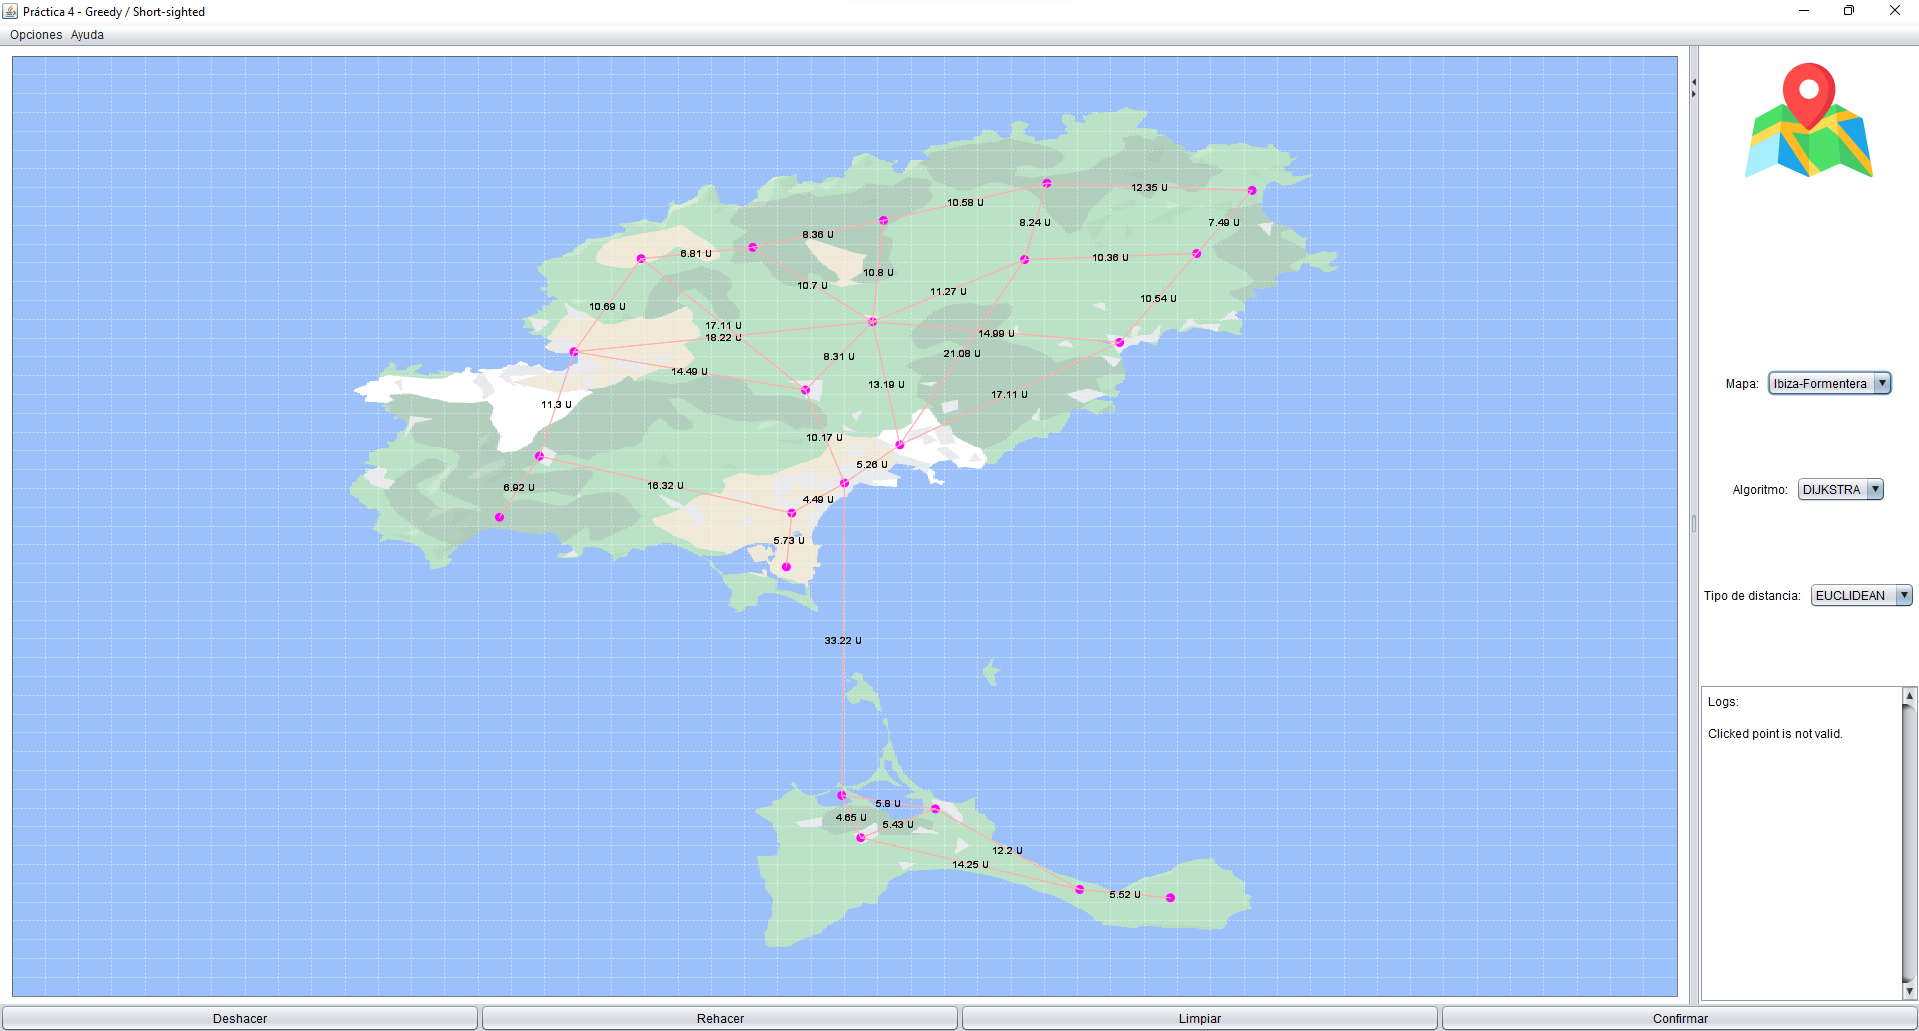
\includegraphics[width=\linewidth]{Usage/img/GUI.png}
    \caption{Interfaz de usuario}
    \label{fig:User_interface}
\end{figure}

\subsection{Header}\label{Manual usuario, Header}
En el \say{header} de la aplicación podemos encontrar un conjunto de botones con imágenes que nos permiten seleccionar las piezas para poner sobre el tablero. Cuando se seleccione una pieza, ésta se verá reflejada en el cursor y se podrá añadir en cualquier punto del tablero clicando sobre una casilla. \bigskip

Los botones del \say{header} para seleccionar las piezas, de izquierda a derecha, son: 

\begin{multicols}{2}
\begin{itemize}
    \item[] Rey
    \item[] Reina
    \item[] Torre
    \item[] Caballo
    \item[] Álfil
    \item[] Unicornio
    \item[] Dragon
    \item[] Castillo
\end{itemize}
\end{multicols}

\subsection{Main}
En el principal bloque de la aplicación se encuentra el tablero donde se ejecutará el algoritmo de backtracking. En esta sección, se representa el tamaño del tablero, las piezas que hay en el tablero y las casillas. \bigskip

Añadir que en la parte derecha del tablero se podrán consultar las estadísticas, donde se da información acerca del tamaño del tablero, piezas que hay sobre el tablero, tiempo transcurrido y progreso del algoritmo. 

\subsection{Sidebar}
En el \say{Sidebar} de la apliación se encuentran las estadísticas del de la ejecución. En estas estadísticas se indica el tamaño del tablero, el número de piezas que hay sobre el tablero, el tiempo transcurrido en encontrar la solución y el progreso del algoritmo se verá reflejado en la barra de progreso.

\subsection{Footer}
En el \say{footer} de la aplicación se pueden encontrar un conjunto de \say{gadgets} que nos permiten controlar la ejecución del programa y visualización. A continuación se explicará cada uno de ellos de izquierda a derecha: \bigskip

Primeramente, el botón definido por la etiqueta \say{Iniciar} permite iniciar el algoritmo con la configuración que el usuario haya elegido, es decir, se iniciará con el tamaño del tablero seleccionado y con N piezas sobre el tablero que el usuario habrá indicado donde comienza cada una. Si se pulsa el botón \say{Iniciar} sin que haya ninguna pieza sobre el tablero, saltará un Error diciendo que no hay piezas suficientes piezas en el tablero.  \bigskip

Por otra parte, el botón definido por la etiqueta \say{Reiniciar} permite reiniciar el algoritmo y el tablero y dejarlo como al principio de la ejecución del programa. El usuario deberá introducir otra configuración de piezas y de tamaño de tablero para volverlo a ejecutar.  \bigskip

Por último, a la derecha de éste hay un objeto JSpinner para seleccionar el \say{Tamaño del tablero}, cada vez que se cambie el tamaño del tablero, el cambio se verá reflejado sobre el tablero representado por pantalla. Como mínimo, el tablero tiene que ser de 2x2 y como máximo 32x32. Queda claro que el algoritmo tardará menos en ejecutarse en un tablero de 2x2 que en un tablero de 32x32, ya que se tienen que recorrer muchos menos puntos.

\subsection{Ejemplo ejecución}

Al iniciar la aplicación se mostrará una interfaz como la expuesta en la imagen \ref{fig:User_interface}. Para poder iniciar la ejecución del algoritmo, es necesario que se coloquen 1 o más piezas en el tablero de diferentes tipos, como se ha mencionado anteriormente en la sección \ref{Manual usuario, Header}. Una vez ya seleccionada las N fichas, se debe pulsar el botón de iniciar, provacando que se inicie el algoritmo y viendo a tiempo real la ejecución del \say{backtracking}, junto a los datos de la ejecución a la derecha.\bigskip

A continuación, la siguiente imagen, muestra un ejemplo de la interfaz en mitad de la ejecución:

\begin{figure}[!h]
    \centering
    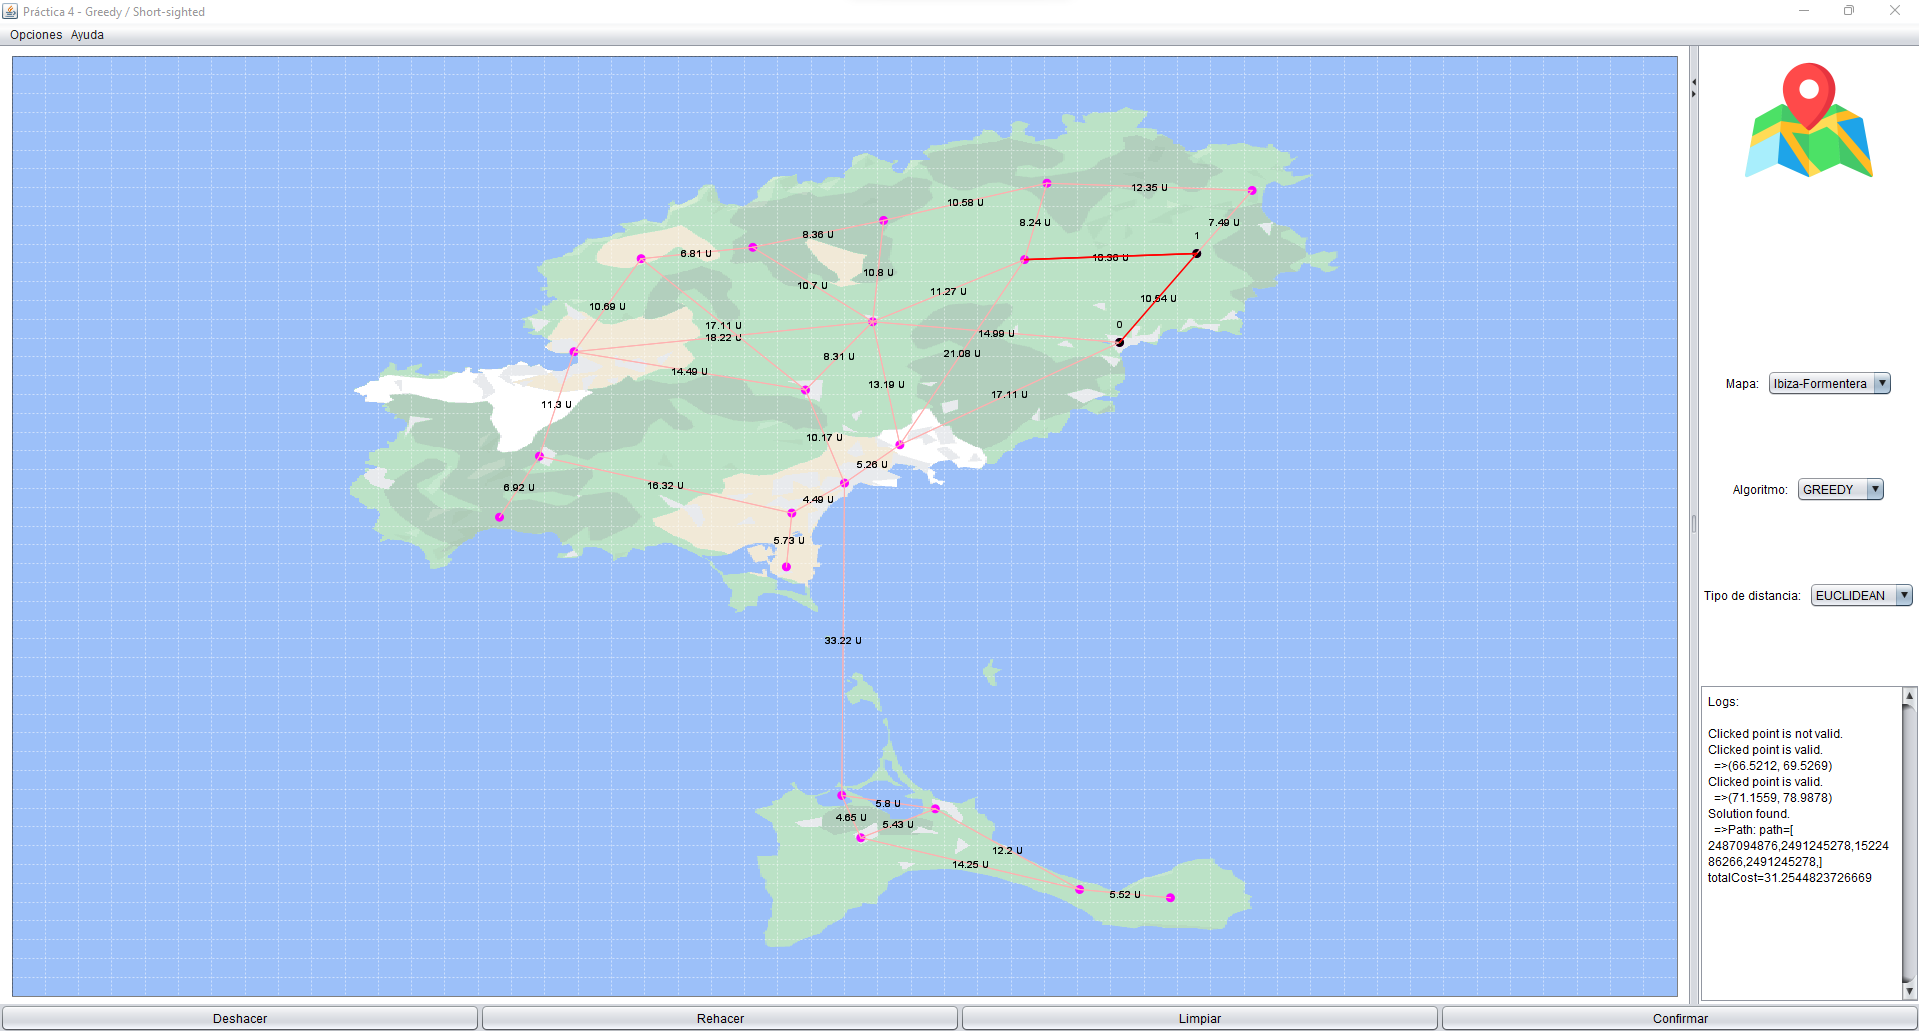
\includegraphics[width=\linewidth]{Usage/img/ejecucion.png}
    \caption{Interfaz de usuario}
    \label{fig:Ejemplo ejecución}
\end{figure}

A partir de aqui, el usuario puede reiniciar la ejecución para ejecutar nuevamente el algoritmo.
\section{Manual de usuario}\label{Manual usuario}

Para el correcto uso de la aplicación, el conjunto de acciones que se pueden realizar en dicho programa serán definidas a continuación. También, la distribución de las secciones de la interfaz junto a su explicación y funcionalidad.\bigskip

Cuando se ejecute el programa por primera vez en la pantalla se debe mostrar la siguiente interfaz de usuario:

\begin{figure}[!h]
    \centering
    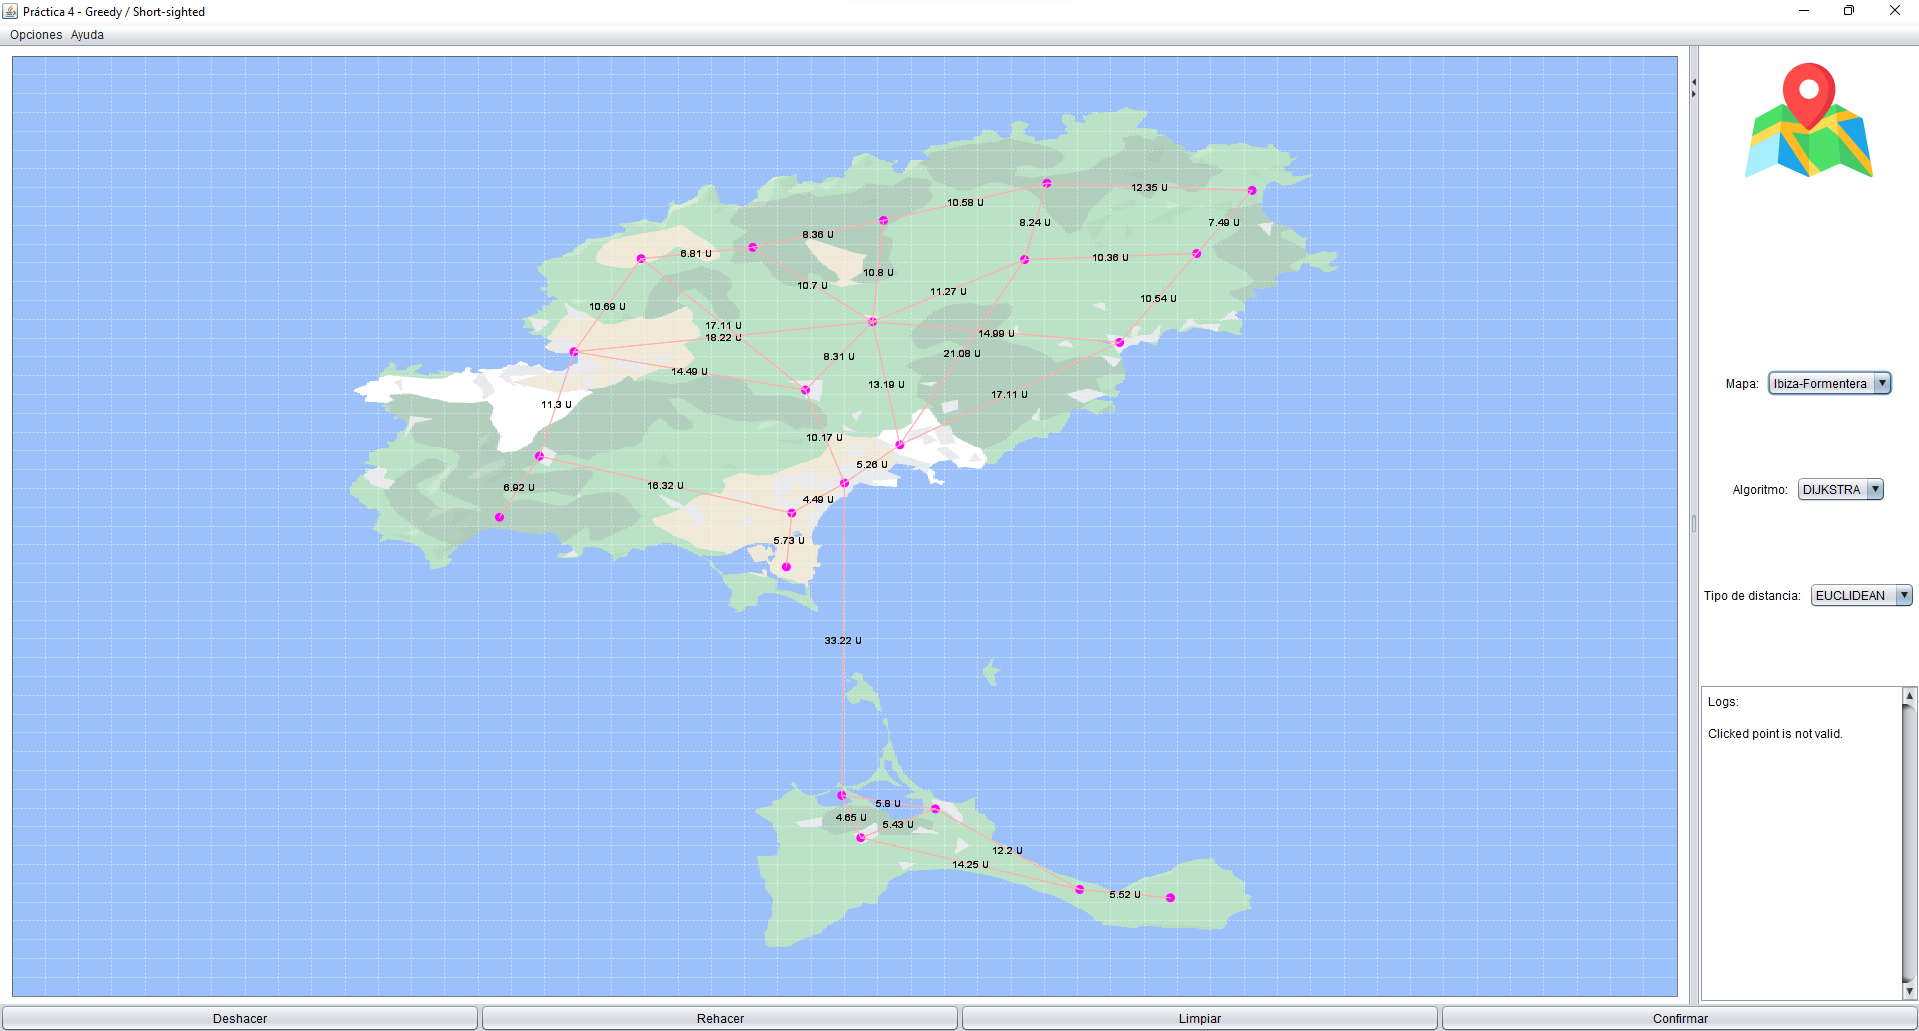
\includegraphics[width=\linewidth]{Usage/img/GUI.png}
    \caption{Interfaz de usuario}
    \label{fig:User_interface}
\end{figure}

\subsection{Header}\label{Manual usuario, Header}
En el \say{header} de la aplicación podemos encontrar un conjunto de botones con imágenes que nos permiten seleccionar las piezas para poner sobre el tablero. Cuando se seleccione una pieza, ésta se verá reflejada en el cursor y se podrá añadir en cualquier punto del tablero clicando sobre una casilla. \bigskip

Los botones del \say{header} para seleccionar las piezas, de izquierda a derecha, son: 

\begin{multicols}{2}
\begin{itemize}
    \item[] Rey
    \item[] Reina
    \item[] Torre
    \item[] Caballo
    \item[] Álfil
    \item[] Unicornio
    \item[] Dragon
    \item[] Castillo
\end{itemize}
\end{multicols}

\subsection{Main}
En el principal bloque de la aplicación se encuentra el tablero donde se ejecutará el algoritmo de backtracking. En esta sección, se representa el tamaño del tablero, las piezas que hay en el tablero y las casillas. \bigskip

Añadir que en la parte derecha del tablero se podrán consultar las estadísticas, donde se da información acerca del tamaño del tablero, piezas que hay sobre el tablero, tiempo transcurrido y progreso del algoritmo. 

\subsection{Sidebar}
En el \say{Sidebar} de la apliación se encuentran las estadísticas del de la ejecución. En estas estadísticas se indica el tamaño del tablero, el número de piezas que hay sobre el tablero, el tiempo transcurrido en encontrar la solución y el progreso del algoritmo se verá reflejado en la barra de progreso.

\subsection{Footer}
En el \say{footer} de la aplicación se pueden encontrar un conjunto de \say{gadgets} que nos permiten controlar la ejecución del programa y visualización. A continuación se explicará cada uno de ellos de izquierda a derecha: \bigskip

Primeramente, el botón definido por la etiqueta \say{Iniciar} permite iniciar el algoritmo con la configuración que el usuario haya elegido, es decir, se iniciará con el tamaño del tablero seleccionado y con N piezas sobre el tablero que el usuario habrá indicado donde comienza cada una. Si se pulsa el botón \say{Iniciar} sin que haya ninguna pieza sobre el tablero, saltará un Error diciendo que no hay piezas suficientes piezas en el tablero.  \bigskip

Por otra parte, el botón definido por la etiqueta \say{Reiniciar} permite reiniciar el algoritmo y el tablero y dejarlo como al principio de la ejecución del programa. El usuario deberá introducir otra configuración de piezas y de tamaño de tablero para volverlo a ejecutar.  \bigskip

Por último, a la derecha de éste hay un objeto JSpinner para seleccionar el \say{Tamaño del tablero}, cada vez que se cambie el tamaño del tablero, el cambio se verá reflejado sobre el tablero representado por pantalla. Como mínimo, el tablero tiene que ser de 2x2 y como máximo 32x32. Queda claro que el algoritmo tardará menos en ejecutarse en un tablero de 2x2 que en un tablero de 32x32, ya que se tienen que recorrer muchos menos puntos.

\subsection{Ejemplo ejecución}

Al iniciar la aplicación se mostrará una interfaz como la expuesta en la imagen \ref{fig:User_interface}. Para poder iniciar la ejecución del algoritmo, es necesario que se coloquen 1 o más piezas en el tablero de diferentes tipos, como se ha mencionado anteriormente en la sección \ref{Manual usuario, Header}. Una vez ya seleccionada las N fichas, se debe pulsar el botón de iniciar, provacando que se inicie el algoritmo y viendo a tiempo real la ejecución del \say{backtracking}, junto a los datos de la ejecución a la derecha.\bigskip

A continuación, la siguiente imagen, muestra un ejemplo de la interfaz en mitad de la ejecución:

\begin{figure}[!h]
    \centering
    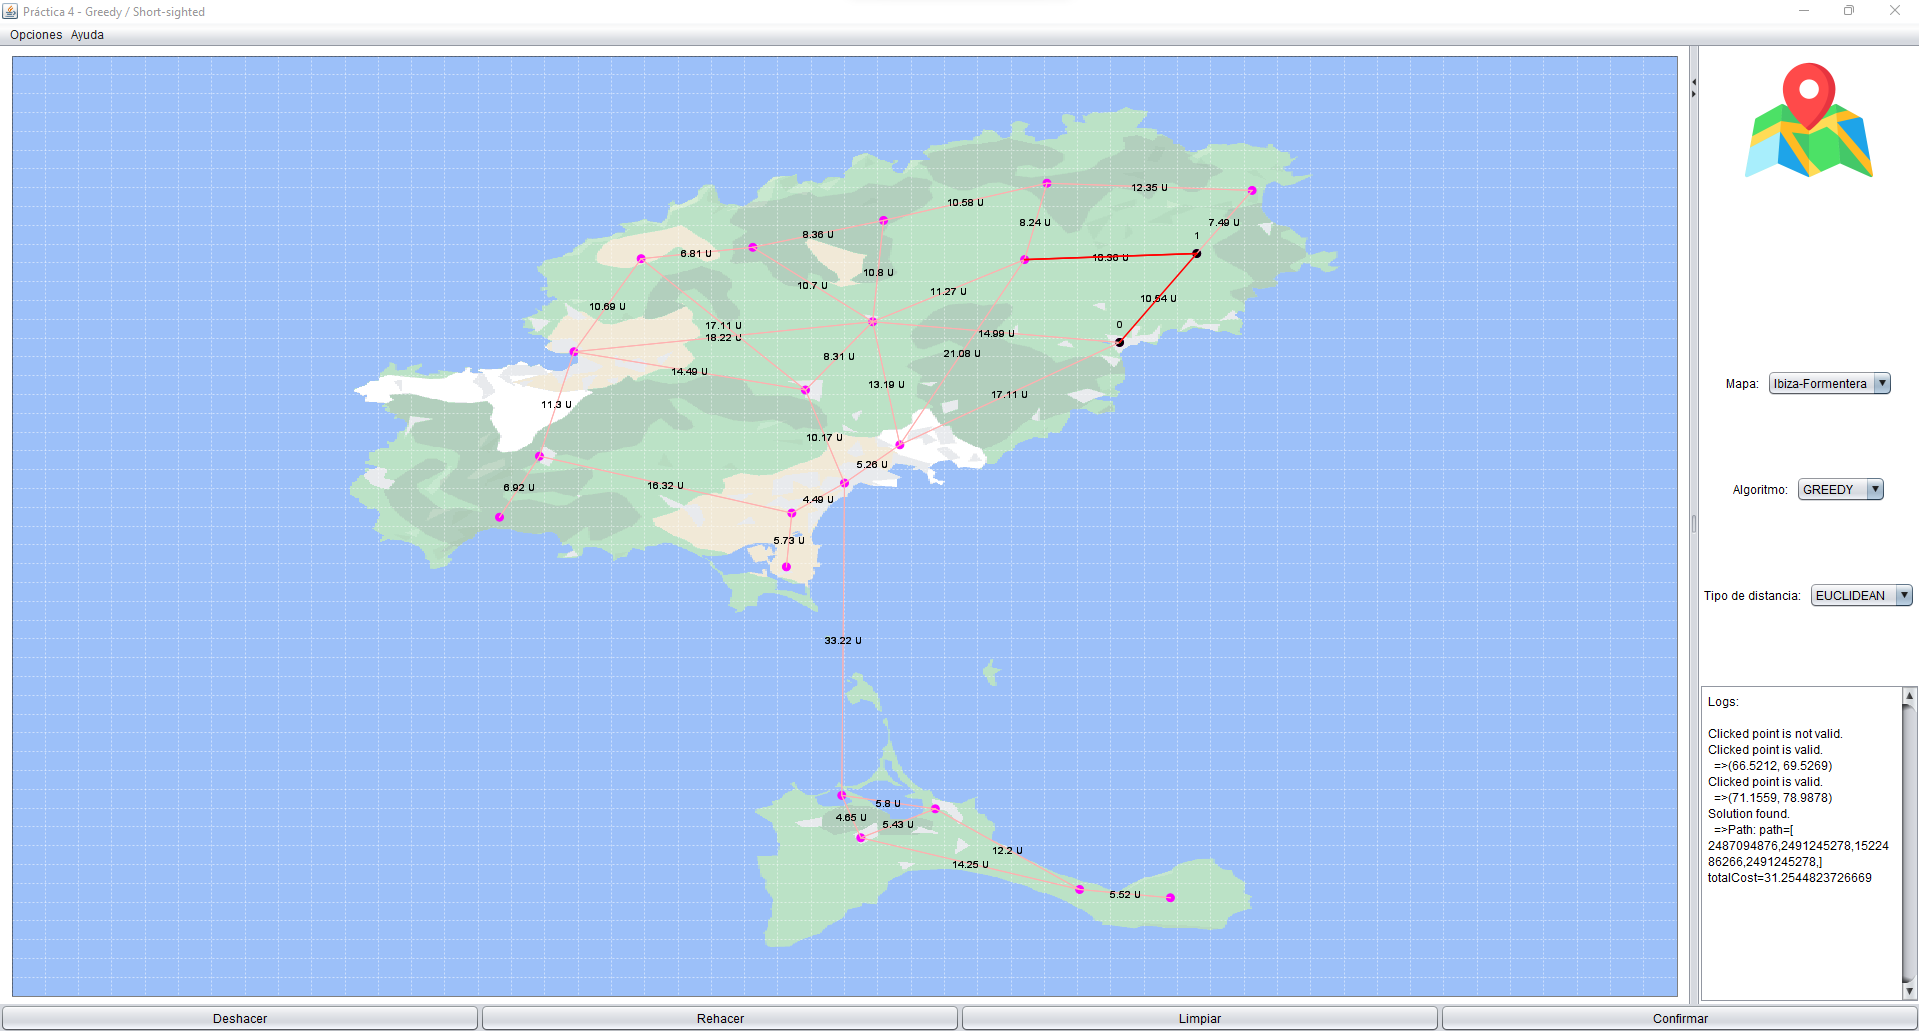
\includegraphics[width=\linewidth]{Usage/img/ejecucion.png}
    \caption{Interfaz de usuario}
    \label{fig:Ejemplo ejecución}
\end{figure}

A partir de aqui, el usuario puede reiniciar la ejecución para ejecutar nuevamente el algoritmo.
\section{Manual de usuario}\label{Manual usuario}

Para el correcto uso de la aplicación, el conjunto de acciones que se pueden realizar en dicho programa serán definidas a continuación. También, la distribución de las secciones de la interfaz junto a su explicación y funcionalidad.\bigskip

Cuando se ejecute el programa por primera vez en la pantalla se debe mostrar la siguiente interfaz de usuario:

\begin{figure}[!h]
    \centering
    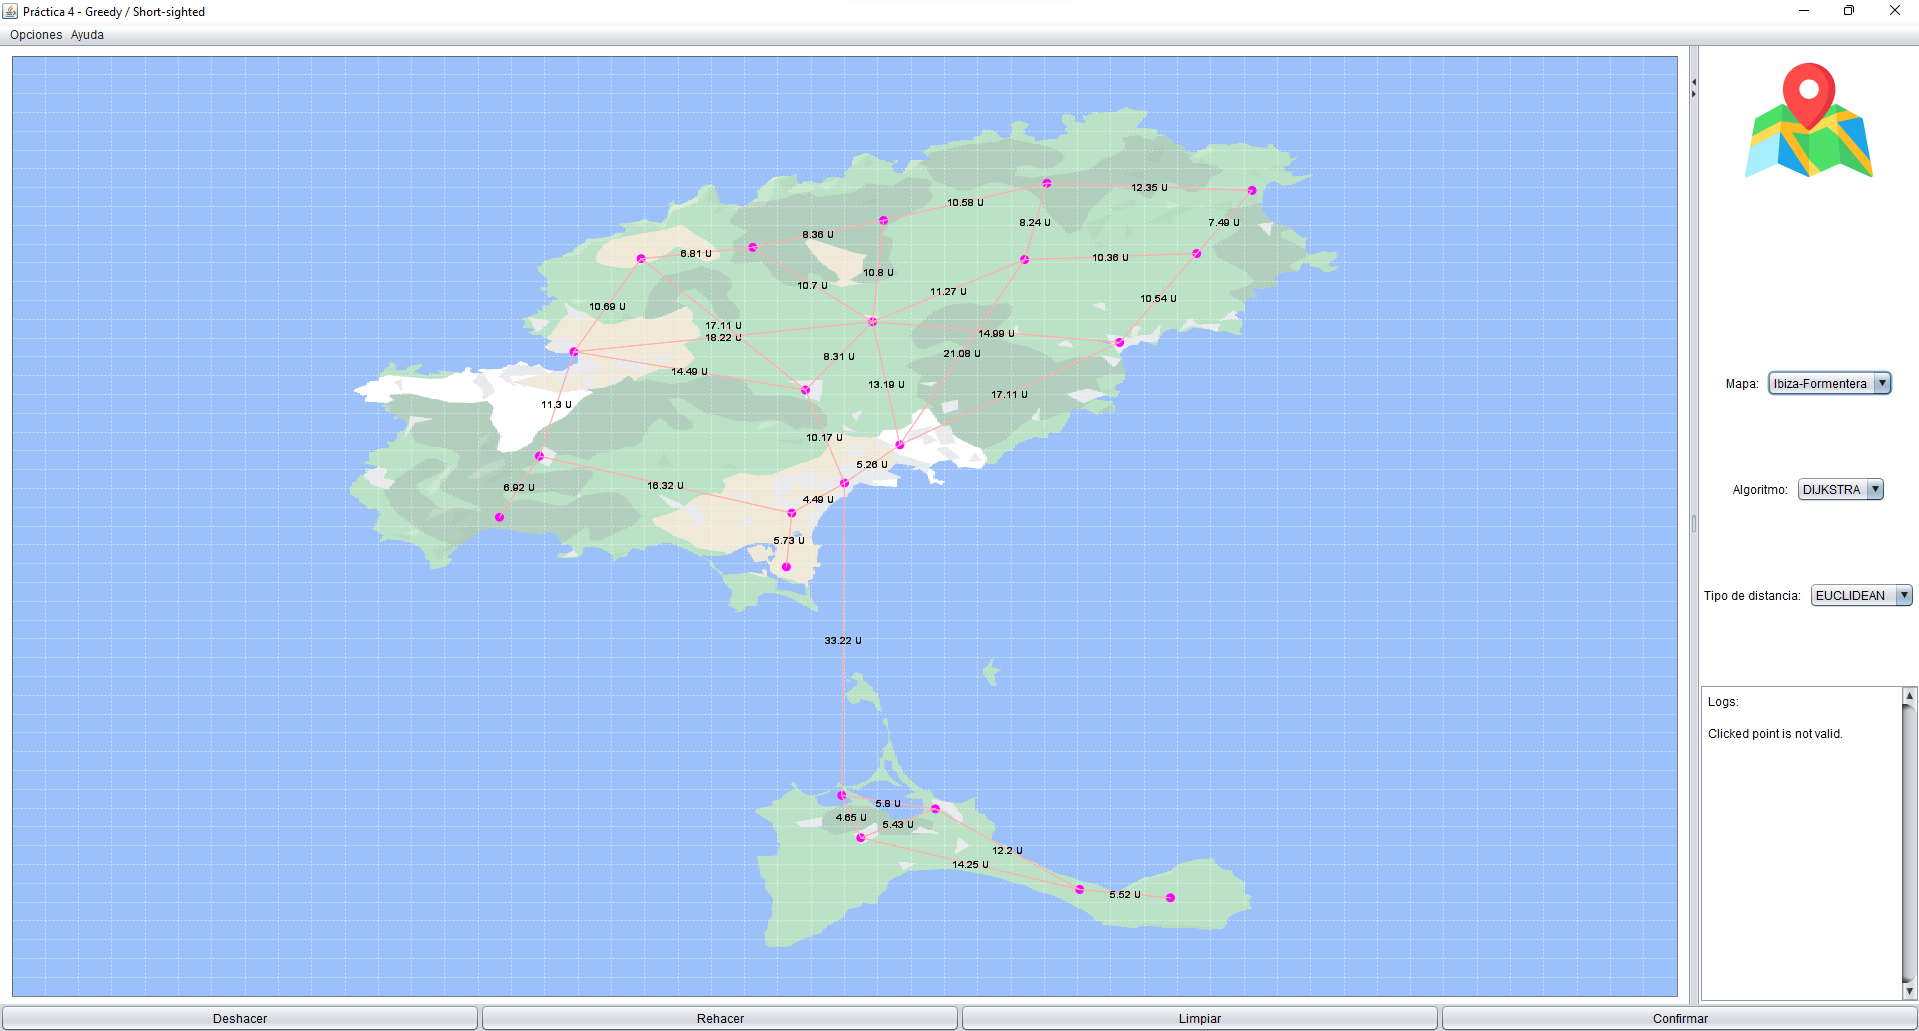
\includegraphics[width=\linewidth]{Usage/img/GUI.png}
    \caption{Interfaz de usuario}
    \label{fig:User_interface}
\end{figure}

\subsection{Header}\label{Manual usuario, Header}
En el \say{header} de la aplicación podemos encontrar un conjunto de botones con imágenes que nos permiten seleccionar las piezas para poner sobre el tablero. Cuando se seleccione una pieza, ésta se verá reflejada en el cursor y se podrá añadir en cualquier punto del tablero clicando sobre una casilla. \bigskip

Los botones del \say{header} para seleccionar las piezas, de izquierda a derecha, son: 

\begin{multicols}{2}
\begin{itemize}
    \item[] Rey
    \item[] Reina
    \item[] Torre
    \item[] Caballo
    \item[] Álfil
    \item[] Unicornio
    \item[] Dragon
    \item[] Castillo
\end{itemize}
\end{multicols}

\subsection{Main}
En el principal bloque de la aplicación se encuentra el tablero donde se ejecutará el algoritmo de backtracking. En esta sección, se representa el tamaño del tablero, las piezas que hay en el tablero y las casillas. \bigskip

Añadir que en la parte derecha del tablero se podrán consultar las estadísticas, donde se da información acerca del tamaño del tablero, piezas que hay sobre el tablero, tiempo transcurrido y progreso del algoritmo. 

\subsection{Sidebar}
En el \say{Sidebar} de la apliación se encuentran las estadísticas del de la ejecución. En estas estadísticas se indica el tamaño del tablero, el número de piezas que hay sobre el tablero, el tiempo transcurrido en encontrar la solución y el progreso del algoritmo se verá reflejado en la barra de progreso.

\subsection{Footer}
En el \say{footer} de la aplicación se pueden encontrar un conjunto de \say{gadgets} que nos permiten controlar la ejecución del programa y visualización. A continuación se explicará cada uno de ellos de izquierda a derecha: \bigskip

Primeramente, el botón definido por la etiqueta \say{Iniciar} permite iniciar el algoritmo con la configuración que el usuario haya elegido, es decir, se iniciará con el tamaño del tablero seleccionado y con N piezas sobre el tablero que el usuario habrá indicado donde comienza cada una. Si se pulsa el botón \say{Iniciar} sin que haya ninguna pieza sobre el tablero, saltará un Error diciendo que no hay piezas suficientes piezas en el tablero.  \bigskip

Por otra parte, el botón definido por la etiqueta \say{Reiniciar} permite reiniciar el algoritmo y el tablero y dejarlo como al principio de la ejecución del programa. El usuario deberá introducir otra configuración de piezas y de tamaño de tablero para volverlo a ejecutar.  \bigskip

Por último, a la derecha de éste hay un objeto JSpinner para seleccionar el \say{Tamaño del tablero}, cada vez que se cambie el tamaño del tablero, el cambio se verá reflejado sobre el tablero representado por pantalla. Como mínimo, el tablero tiene que ser de 2x2 y como máximo 32x32. Queda claro que el algoritmo tardará menos en ejecutarse en un tablero de 2x2 que en un tablero de 32x32, ya que se tienen que recorrer muchos menos puntos.

\subsection{Ejemplo ejecución}

Al iniciar la aplicación se mostrará una interfaz como la expuesta en la imagen \ref{fig:User_interface}. Para poder iniciar la ejecución del algoritmo, es necesario que se coloquen 1 o más piezas en el tablero de diferentes tipos, como se ha mencionado anteriormente en la sección \ref{Manual usuario, Header}. Una vez ya seleccionada las N fichas, se debe pulsar el botón de iniciar, provacando que se inicie el algoritmo y viendo a tiempo real la ejecución del \say{backtracking}, junto a los datos de la ejecución a la derecha.\bigskip

A continuación, la siguiente imagen, muestra un ejemplo de la interfaz en mitad de la ejecución:

\begin{figure}[!h]
    \centering
    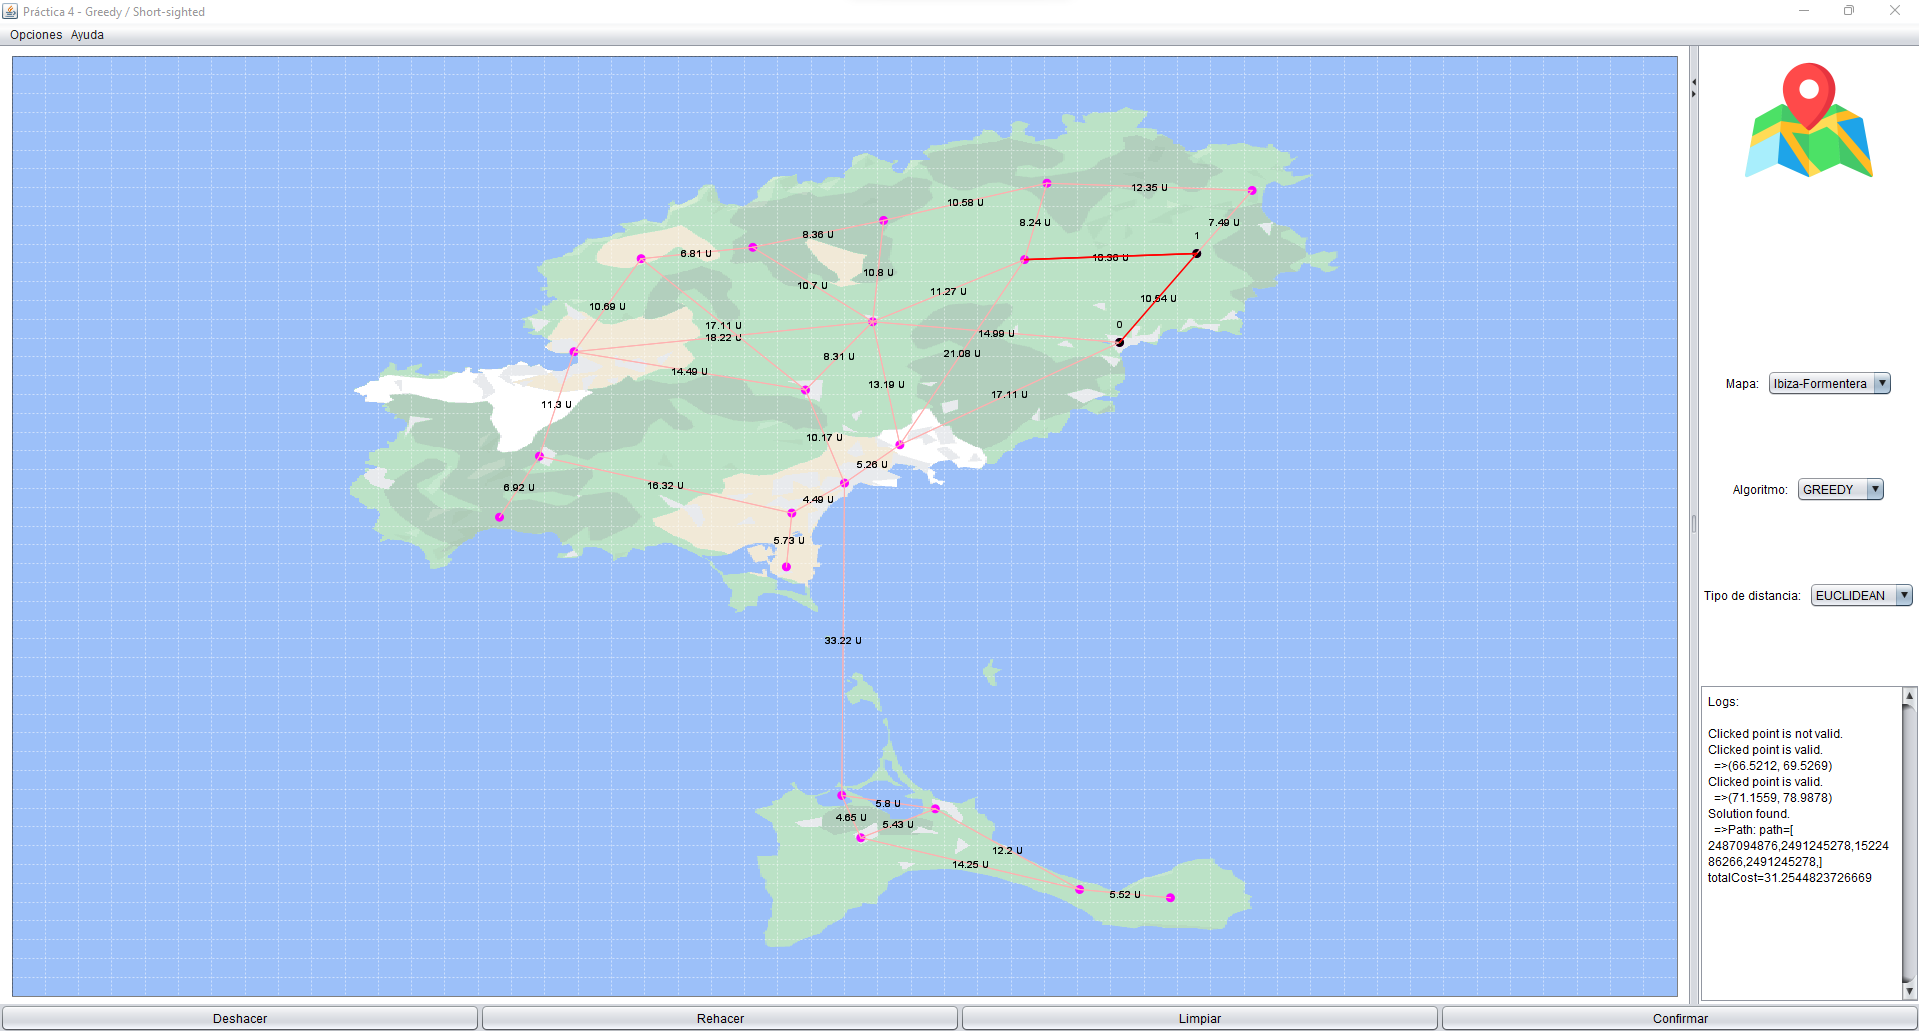
\includegraphics[width=\linewidth]{Usage/img/ejecucion.png}
    \caption{Interfaz de usuario}
    \label{fig:Ejemplo ejecución}
\end{figure}

A partir de aqui, el usuario puede reiniciar la ejecución para ejecutar nuevamente el algoritmo.
\section{Manual de usuario}\label{Manual usuario}

Para el correcto uso de la aplicación, el conjunto de acciones que se pueden realizar en dicho programa serán definidas a continuación. También, la distribución de las secciones de la interfaz junto a su explicación y funcionalidad.\bigskip

Cuando se ejecute el programa por primera vez en la pantalla se debe mostrar la siguiente interfaz de usuario:

\begin{figure}[!h]
    \centering
    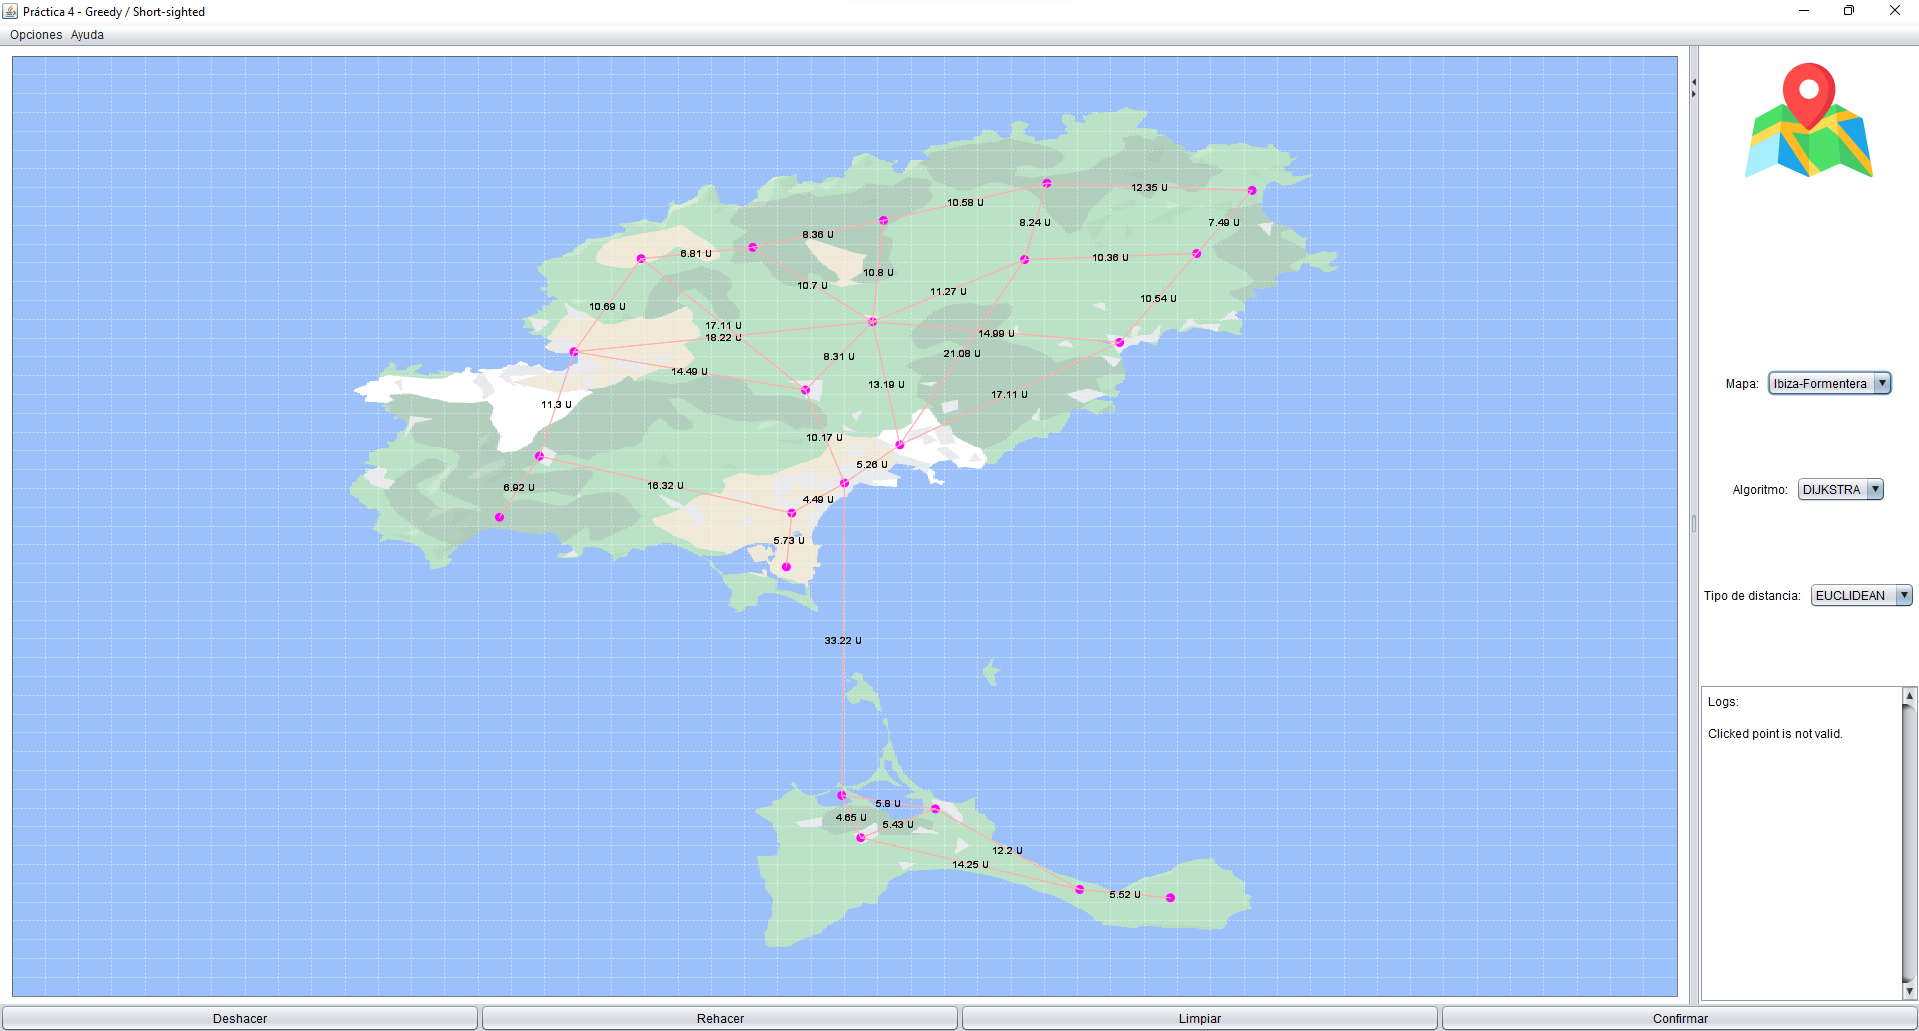
\includegraphics[width=\linewidth]{Usage/img/GUI.png}
    \caption{Interfaz de usuario}
    \label{fig:User_interface}
\end{figure}

\subsection{Header}\label{Manual usuario, Header}
En el \say{header} de la aplicación podemos encontrar un conjunto de botones con imágenes que nos permiten seleccionar las piezas para poner sobre el tablero. Cuando se seleccione una pieza, ésta se verá reflejada en el cursor y se podrá añadir en cualquier punto del tablero clicando sobre una casilla. \bigskip

Los botones del \say{header} para seleccionar las piezas, de izquierda a derecha, son: 

\begin{multicols}{2}
\begin{itemize}
    \item[] Rey
    \item[] Reina
    \item[] Torre
    \item[] Caballo
    \item[] Álfil
    \item[] Unicornio
    \item[] Dragon
    \item[] Castillo
\end{itemize}
\end{multicols}

\subsection{Main}
En el principal bloque de la aplicación se encuentra el tablero donde se ejecutará el algoritmo de backtracking. En esta sección, se representa el tamaño del tablero, las piezas que hay en el tablero y las casillas. \bigskip

Añadir que en la parte derecha del tablero se podrán consultar las estadísticas, donde se da información acerca del tamaño del tablero, piezas que hay sobre el tablero, tiempo transcurrido y progreso del algoritmo. 

\subsection{Sidebar}
En el \say{Sidebar} de la apliación se encuentran las estadísticas del de la ejecución. En estas estadísticas se indica el tamaño del tablero, el número de piezas que hay sobre el tablero, el tiempo transcurrido en encontrar la solución y el progreso del algoritmo se verá reflejado en la barra de progreso.

\subsection{Footer}
En el \say{footer} de la aplicación se pueden encontrar un conjunto de \say{gadgets} que nos permiten controlar la ejecución del programa y visualización. A continuación se explicará cada uno de ellos de izquierda a derecha: \bigskip

Primeramente, el botón definido por la etiqueta \say{Iniciar} permite iniciar el algoritmo con la configuración que el usuario haya elegido, es decir, se iniciará con el tamaño del tablero seleccionado y con N piezas sobre el tablero que el usuario habrá indicado donde comienza cada una. Si se pulsa el botón \say{Iniciar} sin que haya ninguna pieza sobre el tablero, saltará un Error diciendo que no hay piezas suficientes piezas en el tablero.  \bigskip

Por otra parte, el botón definido por la etiqueta \say{Reiniciar} permite reiniciar el algoritmo y el tablero y dejarlo como al principio de la ejecución del programa. El usuario deberá introducir otra configuración de piezas y de tamaño de tablero para volverlo a ejecutar.  \bigskip

Por último, a la derecha de éste hay un objeto JSpinner para seleccionar el \say{Tamaño del tablero}, cada vez que se cambie el tamaño del tablero, el cambio se verá reflejado sobre el tablero representado por pantalla. Como mínimo, el tablero tiene que ser de 2x2 y como máximo 32x32. Queda claro que el algoritmo tardará menos en ejecutarse en un tablero de 2x2 que en un tablero de 32x32, ya que se tienen que recorrer muchos menos puntos.

\subsection{Ejemplo ejecución}

Al iniciar la aplicación se mostrará una interfaz como la expuesta en la imagen \ref{fig:User_interface}. Para poder iniciar la ejecución del algoritmo, es necesario que se coloquen 1 o más piezas en el tablero de diferentes tipos, como se ha mencionado anteriormente en la sección \ref{Manual usuario, Header}. Una vez ya seleccionada las N fichas, se debe pulsar el botón de iniciar, provacando que se inicie el algoritmo y viendo a tiempo real la ejecución del \say{backtracking}, junto a los datos de la ejecución a la derecha.\bigskip

A continuación, la siguiente imagen, muestra un ejemplo de la interfaz en mitad de la ejecución:

\begin{figure}[!h]
    \centering
    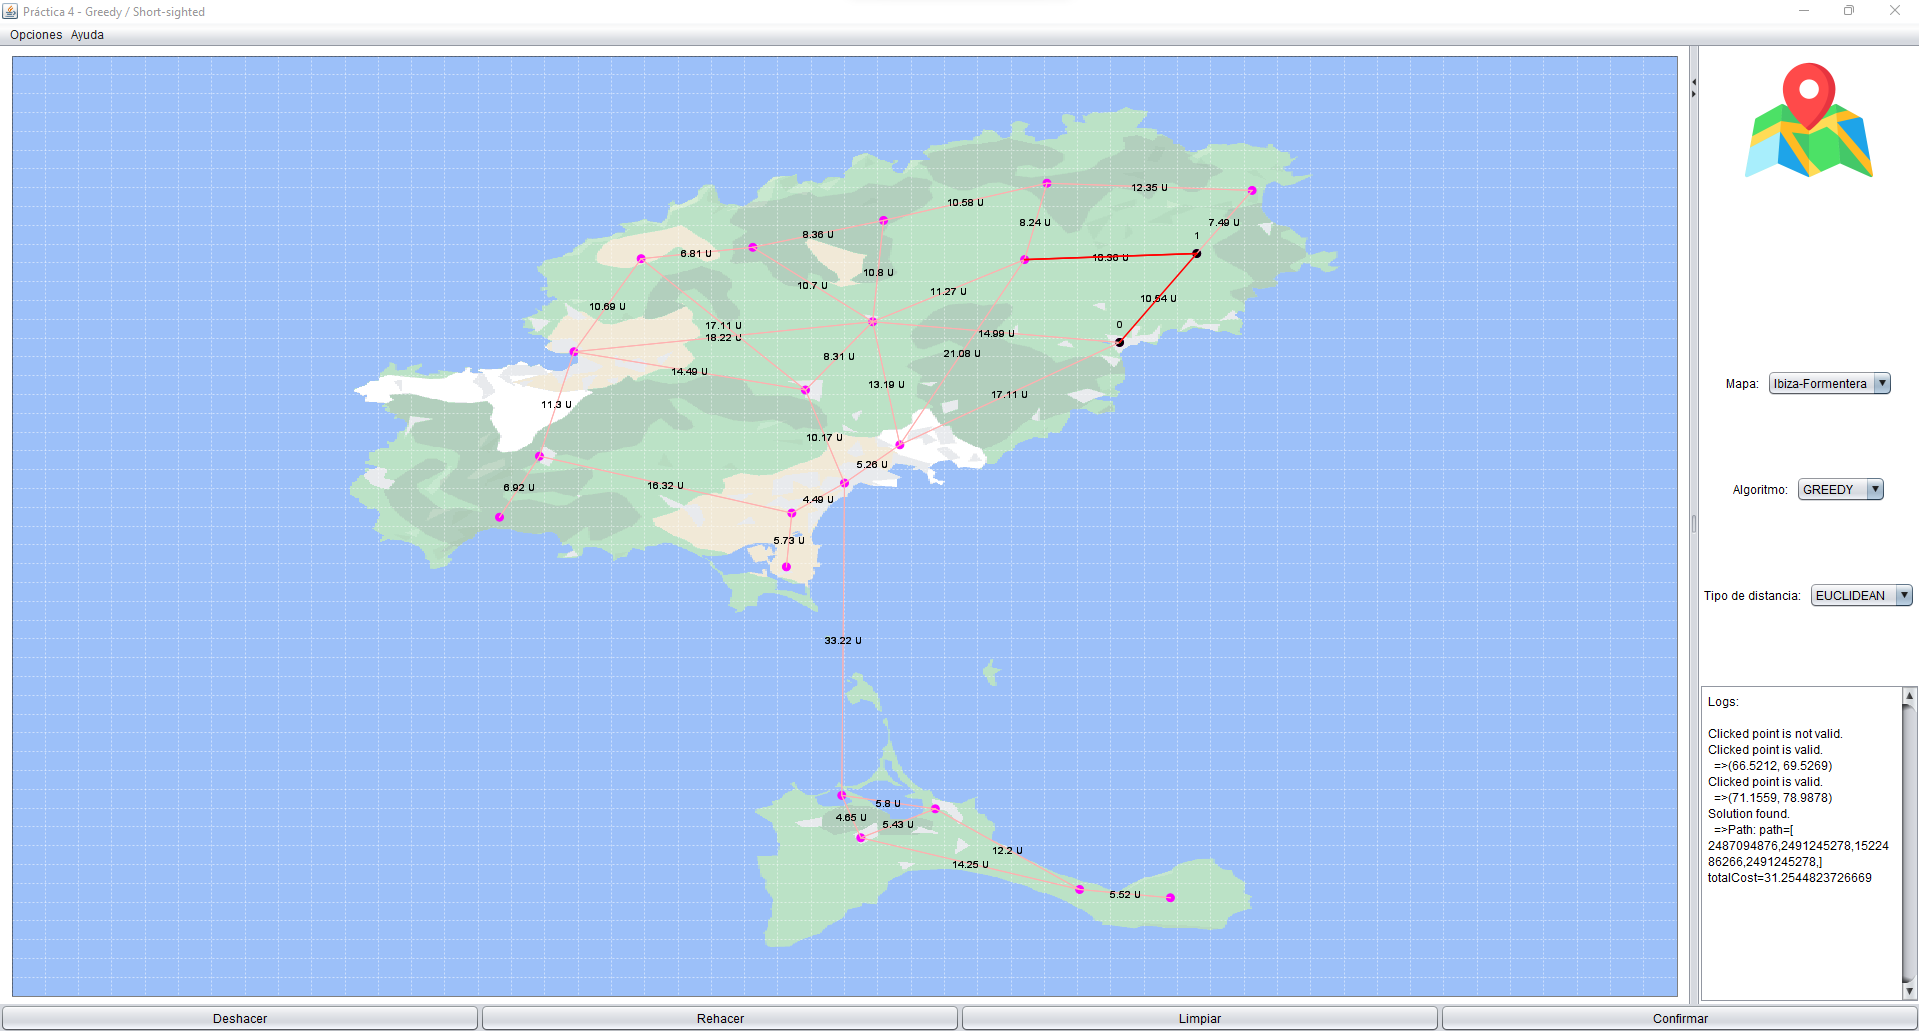
\includegraphics[width=\linewidth]{Usage/img/ejecucion.png}
    \caption{Interfaz de usuario}
    \label{fig:Ejemplo ejecución}
\end{figure}

A partir de aqui, el usuario puede reiniciar la ejecución para ejecutar nuevamente el algoritmo.
